% Created 2023-05-16 Tue 10:42
% Intended LaTeX compiler: pdflatex
\documentclass[aspectratio=169,t]{beamer}
\usepackage[utf8]{inputenc}
\usepackage[T1]{fontenc}
\usepackage{graphicx}
\usepackage{longtable}
\usepackage{wrapfig}
\usepackage{rotating}
\usepackage[normalem]{ulem}
\usepackage{amsmath}
\usepackage{amssymb}
\usepackage{capt-of}
\usepackage{hyperref}
\usepackage{listings}
\usepackage{ccicons}
\usepackage[margin=3pt,font=scriptsize,labelfont=bf]{caption}
\usepackage{animate}
\usepackage{svg}
\usepackage{mathtools}
\DeclarePairedDelimiter\abs{\lvert}{\rvert} % ABS: abs{}
\newenvironment{asvector}{\left\langle\begin{smallmatrix}}{\end{smallmatrix}\right\rangle}
\newenvironment{avector}{\left\langle\begin{matrix}}{\end{matrix}\right\rangle}
\newenvironment{talign*}{\centering $\displaystyle\begin{aligned}}{\end{aligned}$\par}
\usetheme{focus}
\author{Samuel J Monson}
\date{2023-05-16}
\title{Complex and Hypercomplex \\ Iterative Methods}
\institute{Seattle Univerisity}
\definecolor{main}{HTML}{93361f}
\definecolor{background}{HTML}{D0D0D0}
\definecolor{royalblue}{HTML}{4169e1}
\definecolor{forestgreen}{HTML}{228b22}
\setmathfont{Fira Math}
\setmathfont{DejaVu Math TeX Gyre}[range={\vysmwhtcircle,\times,\vdots}]
\setmonofont{Hack}
\hypersetup{
 pdfauthor={Samuel J Monson},
 pdftitle={Complex and Hypercomplex \\ Iterative Methods},
 pdfkeywords={},
 pdfsubject={},
 pdfcreator={Emacs 30.0.50 (Org mode 9.6.1)}, 
 pdflang={English}}
\begin{document}

\begin{frame}
\maketitle
\end{frame}
\begin{frame}{Outline}
\setcounter{tocdepth}{2}
\tableofcontents
\end{frame}

\begin{frame}[label={sec:org0af5b08}]{Definitions}
\begin{definition}[Iterative Method]\label{sec:org7c6b3f5}
A sequence where each value in the sequence is defined by the previous value.
\end{definition}

\begin{definition}<2->[Dynamical System]\label{sec:org690275f}
A system that enacts rules on a set of variables to produce a state.
\end{definition}

\begin{definition}<3->[Complex Dynamics]\label{sec:org590f4e4}
The study of \uline{dynamical systems} defined by complex functions.
\end{definition}
\end{frame}

\section{Iteration}
\label{sec:orgce3a066}

\begin{frame}[label={sec:orga2edc22}]{Iteration}
\begin{definition}[Function Iteration]\label{sec:orgbeb6ea4}
\(f^0 := \symbf{I}\)

\(f^{k+1} := f \circ f^k\)
\end{definition}

\begin{exampleblock}<2->{Example}\label{sec:orgf54d97f}
Given \(f(x) = x + 1\),

\begin{talign*}
    \onslide<3->{f^0(x) & = x \\}
    \onslide<4->{f^1(x) & = x + 1 \\}
    \onslide<5->{f^2(x) & = (x + 1) + 1 \\}
    \onslide<6->{f^3(x) & = \left((x + 1) + 1\right) + 1 \\}
    \onslide<6->{\vdots}
\end{talign*}
\end{exampleblock}
\end{frame}

\section{Complex Iterative Methods}
\label{sec:orgb7e2323}

\begin{frame}[label={sec:org778eff3}]{Complex Numbers}
\begin{definition}[Complex Numbers]\label{sec:org0e275cc}
\(\symbf{i}^2 = -1\)

\(\{a + b \symbf{i} : a,b \in \symbb{R} \} \in \symbb{C}\)
\end{definition}

\begin{columns}
\begin{column}{0.5\columnwidth}
\begin{block}<2->{Addition}
Let \(a,b,x,y \in \symbb{R}\),

\vspace{\baselineskip}
\begin{talign*}
    (a + b\symbf{i}) + (x + y\symbf{i}) \onslide<4->{& = (a + x) + (b + y)\symbf{i}}
\end{talign*}
\end{block}
\end{column}

\begin{column}{0.5\columnwidth}
\begin{block}<5->{Multiplication}
Let \(a,b,x,y \in \symbb{R}\),

\vspace{\baselineskip}
\begin{talign*}
    (a + b\symbf{i}) \ast (x + y\symbf{i}) \onslide<7->{& = ax + ay\symbf{i} + bx\symbf{i} + by\symbf{i}^2 \\}
    \onslide<8->{& = (ax - by) + (ay + bx)\symbf{i}}
\end{talign*}
\end{block}
\end{column}
\end{columns}
\end{frame}

\begin{frame}[label={sec:org149ed43}]{Complex Iteration}
\begin{columns}
\begin{column}{0.5\columnwidth}
\begin{block}{Rules}
\(f(z) = z^2\)

\(z_0 = \frac{1}{\sqrt{2}} + \frac{1}{\sqrt{2}} \symbf{i}\)
\end{block}

\begin{itemize}[<+->]
\item \(f^0(z) = \frac{1}{\sqrt{2}} + \frac{1}{\sqrt{2}} \symbf{i}\)
\item \(f^1(z) \only<2>{= \left( \frac{1}{\sqrt{2}} + \frac{1}{\sqrt{2}} \symbf{i} \right)^2 = \left( \frac{1}{\sqrt{2}} \right)^2 - \left(\frac{1}{\sqrt{2}} + \frac{1}{\sqrt{2}}\right)^2 + \left(\frac{1}{\sqrt{2}} + \frac{1}{\sqrt{2}}\right)^2 \symbf{i}} = \symbf{i}\)
\item \(f^2(z) = -1\)
\item \(f^3(z) = 1\)
\item \(f^4(z) = f^5(z) = f^6(z) = 1\)
\end{itemize}
\end{column}

\begin{column}{0.5\columnwidth}
\begin{center}
\includegraphics<1>[width=.9\linewidth]{Figs/exports/Iter_1-0.png}
\includegraphics<2>[width=.9\linewidth]{Figs/exports/Iter_1-1.png}
\includegraphics<3>[width=.9\linewidth]{Figs/exports/Iter_1-2.png}
\includegraphics<4->[width=.9\linewidth]{Figs/exports/Iter_1-3.png}
\end{center}
\end{column}
\end{columns}
\end{frame}

\begin{frame}[label={sec:org6155f5a}]{Complex Iteration}
\begin{columns}
\begin{column}{0.5\columnwidth}
\begin{block}{Rules}
\(f(z) = z^2 - \frac{1}{10} - \frac{1}{10} \symbf{i}\)

\(z_0 = \frac{1}{\sqrt{2}} + \frac{1}{\sqrt{2}} \symbf{i}\)
\end{block}

\begin{itemize}[<+->]
\item \(f^0(z) = \frac{1}{\sqrt{2}} + \frac{1}{\sqrt{2}} \symbf{i}\)
\item \(f^1(z) \only<2>{= -\frac{1}{10} + \left(1 - \frac{1}{10}\right)\symbf{i}} = -0.1 + 0.9\symbf{i}\)
\item \(f^2(z) = -0.9-0.28\symbf{i}\)
\item \(f^3(z) = 0.6316+0.404\symbf{i}\)
\item \(f^4(z) \approx 0.13570256+0.4103328\symbf{i}\)
\item \(f^5(z) \approx -0.24995782+0.01136642\symbf{i}\)
\item \(f^6(z) \approx -0.03765028-0.10568225\symbf{i}\)
\end{itemize}
\end{column}

\begin{column}{0.5\columnwidth}
\begin{center}
\includegraphics<1>[width=.9\linewidth]{Figs/exports/Iter_2-0.png}
\includegraphics<2>[width=.9\linewidth]{Figs/exports/Iter_2-1.png}
\includegraphics<3>[width=.9\linewidth]{Figs/exports/Iter_2-2.png}
\includegraphics<4>[width=.9\linewidth]{Figs/exports/Iter_2-3.png}
\includegraphics<5>[width=.9\linewidth]{Figs/exports/Iter_2-4.png}
\includegraphics<6>[width=.9\linewidth]{Figs/exports/Iter_2-5.png}
\includegraphics<7->[width=.9\linewidth]{Figs/exports/Iter_2-6.png}
\end{center}
\end{column}
\end{columns}
\end{frame}

\begin{frame}[label={sec:org47c96f6}]{Group Activity}
\begin{columns}
\begin{column}{0.5\columnwidth}
\begin{block}{Easier}
\(f(z) = z^2 - 0.2 + 0 \symbf{i}\)

\(z_0 = 0.5 + 0 \symbf{i}\)
\end{block}
\end{column}

\begin{column}{0.5\columnwidth}
\begin{block}{Harder}
\(f(z) = z^2 -0.2 + 0.4 \symbf{i}\)

\(z_0 = 0.5 - 0.5 \symbf{i}\)
\end{block}
\end{column}
\end{columns}
\end{frame}

\begin{frame}[label={sec:org22beed2}]{Group Activity (Easier)}
\begin{columns}
\begin{column}{0.5\columnwidth}
\begin{block}{Rules}
\(f(z) = z^2 -0.2 + 0 \symbf{i}\)

\(z_0 = 0.5 + 0 \symbf{i}\)
\end{block}

\begin{itemize}[<+->]
\item \(f^0(z) = 0.5\)
\item \(f^1(z) = 0.05\)
\item \(f^2(z) = -0.1975\)
\item \(f^3(z) = -0.16099375\)
\item \(f^4(z) \approx -0.1740810125\)
\end{itemize}
\end{column}

\begin{column}{0.5\columnwidth}
\begin{center}
\includegraphics<1>[width=.9\linewidth]{Figs/exports/Iter_3-0.png}
\includegraphics<2>[width=.9\linewidth]{Figs/exports/Iter_3-1.png}
\includegraphics<3>[width=.9\linewidth]{Figs/exports/Iter_3-2.png}
\includegraphics<4>[width=.9\linewidth]{Figs/exports/Iter_3-3.png}
\includegraphics<5->[width=.9\linewidth]{Figs/exports/Iter_3-4.png}
\end{center}
\end{column}
\end{columns}
\end{frame}

\begin{frame}[label={sec:org281c5f8}]{Group Activity (Harder)}
\begin{columns}
\begin{column}{0.5\columnwidth}
\begin{block}{Rules}
\(f(z) = z^2 -0.2 + 0.4 \symbf{i}\)

\(z_0 = 0.5 - 0.5 \symbf{i}\)
\end{block}

\begin{itemize}[<+->]
\item \(f^0(z) = 0.5 - 0.5 \symbf{i}\)
\item \(f^1(z) = -0.2 - 0.1 \symbf{i}\)
\item \(f^2(z) = -0.17 + 0.44 \symbf{i}\)
\item \(f^3(z) = -0.3647 + 0.2504 \symbf{i}\)
\item \(f^4(z) = -0.12969407 + 0.21735824 \symbf{i}\)
\end{itemize}
\end{column}

\begin{column}{0.5\columnwidth}
\begin{center}
\includegraphics<1>[width=.9\linewidth]{Figs/exports/Iter_4-0.png}
\includegraphics<2>[width=.9\linewidth]{Figs/exports/Iter_4-1.png}
\includegraphics<3>[width=.9\linewidth]{Figs/exports/Iter_4-2.png}
\includegraphics<4>[width=.9\linewidth]{Figs/exports/Iter_4-3.png}
\includegraphics<5->[width=.9\linewidth]{Figs/exports/Iter_4-4.png}
\end{center}
\end{column}
\end{columns}
\end{frame}

\begin{frame}[label={sec:orgef336bc},fragile]{Implementation}
 \begin{columns}
\begin{column}{0.50\columnwidth}
\begin{block}{Iteration (Python)}
\begin{lstlisting}[language=Python,firstnumber=1,numbers=left]
N = 128
B = 4
c = complex(-0.2, 0.4)
def iterate(z):
    for n in range(N):
        z = z*z + c
        if abs(z) > B*B: break
    return n
\end{lstlisting}
\end{block}
\end{column}

\begin{column}{0.45\columnwidth}
\begin{center}
\includegraphics<2->[width=.9\linewidth]{Figs/exports/Iter_4-128.png}
\end{center}
\end{column}
\end{columns}
\end{frame}

\begin{frame}[label={sec:orgec879ce}]{Iterative Fractals}
\begin{columns}
\begin{column}{0.55\columnwidth}
\begin{block}{Complex Juila Set Example}
Defined by iterative function in complex space

\begin{itemize}
\item \(f_c (z) = z^2 - 0.675 - 0.112\symbf{i}\)

\item \(K_c = \left\{ z_0 \in \symbb{C}: \abs{f^k_c \left(z_0 \right)} > B \text{ as } k \to \infty\right\}\)
\end{itemize}
\end{block}
\end{column}

\begin{column}{0.45\columnwidth}
\begin{figure}[htbp]
\centering
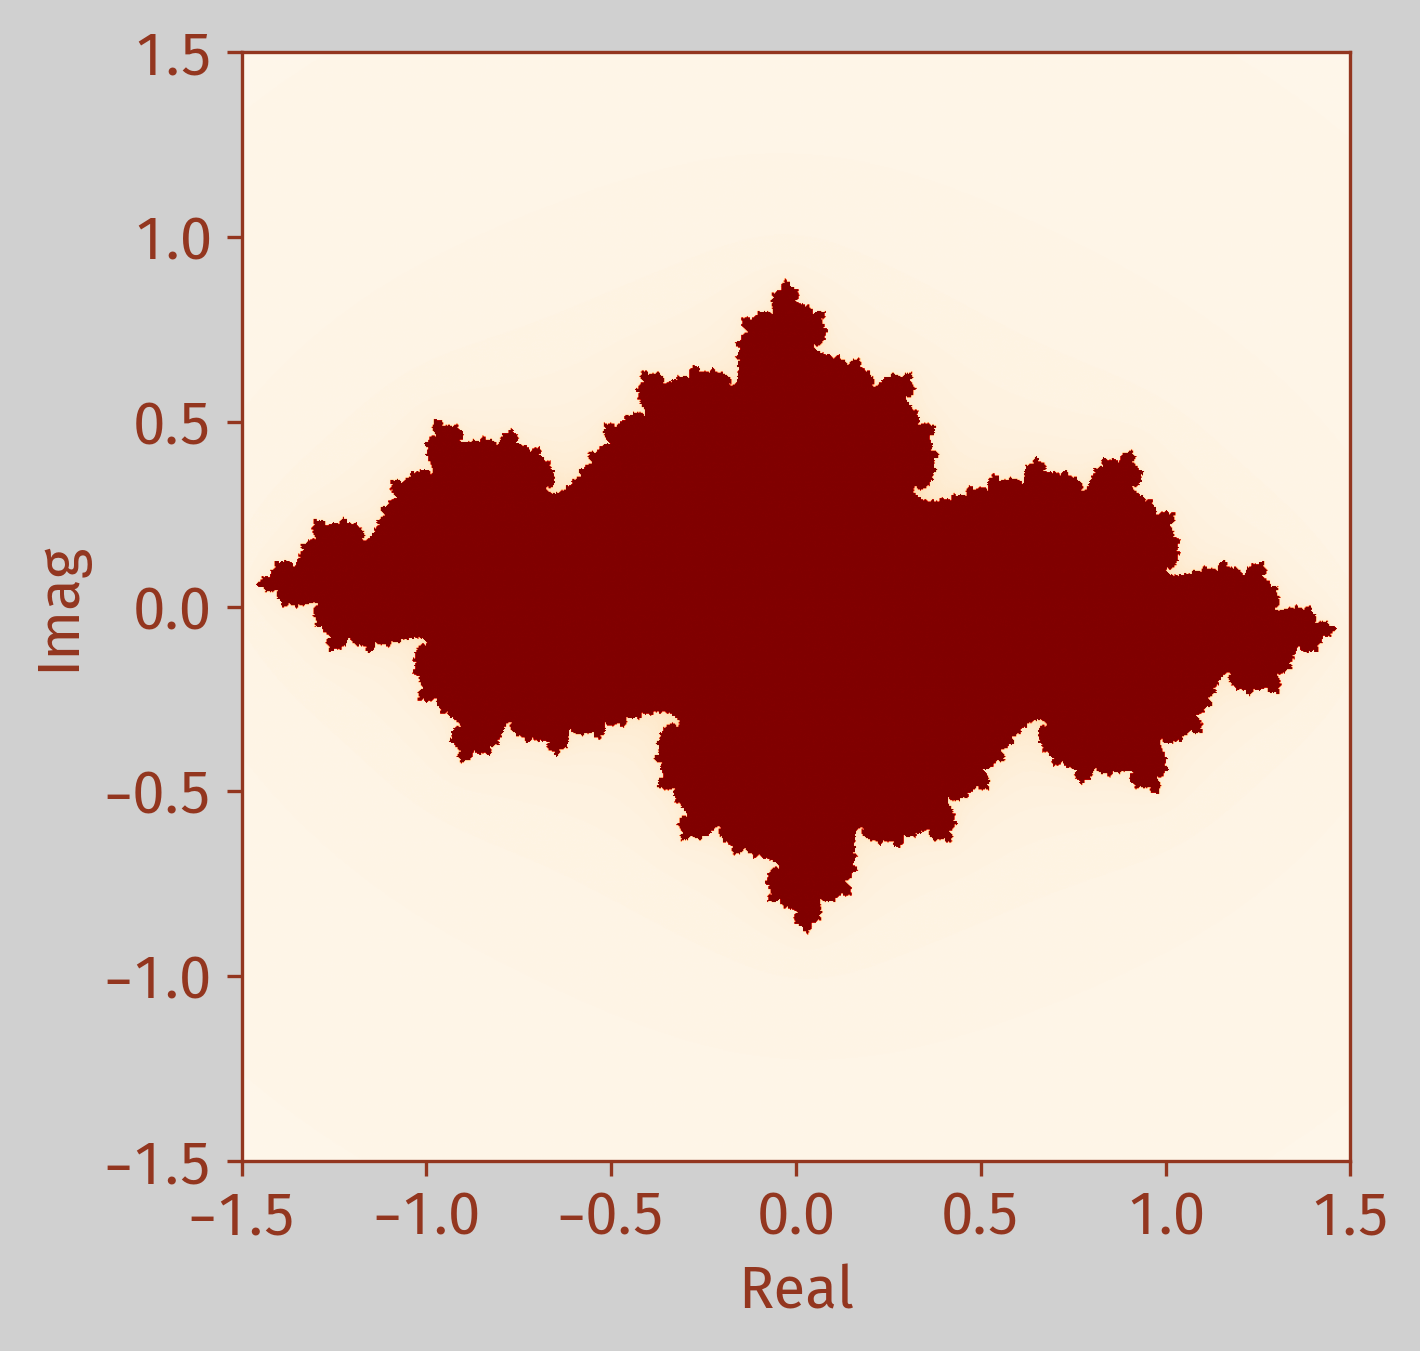
\includegraphics[width=0.80\textwidth]{./Figs/Fig_2v2.png}
\caption{\(f(z) = z^2 -0.675 - 0.112\symbf{i}\)}
\end{figure}
\end{column}
\end{columns}
\end{frame}

\section{Quaternions}
\label{sec:orgf569e58}

\begin{frame}[label={sec:org875eb00},b]{Quaternions History}
\begin{columns}
\begin{column}{0.50\columnwidth}
\begin{figure}[htbp]

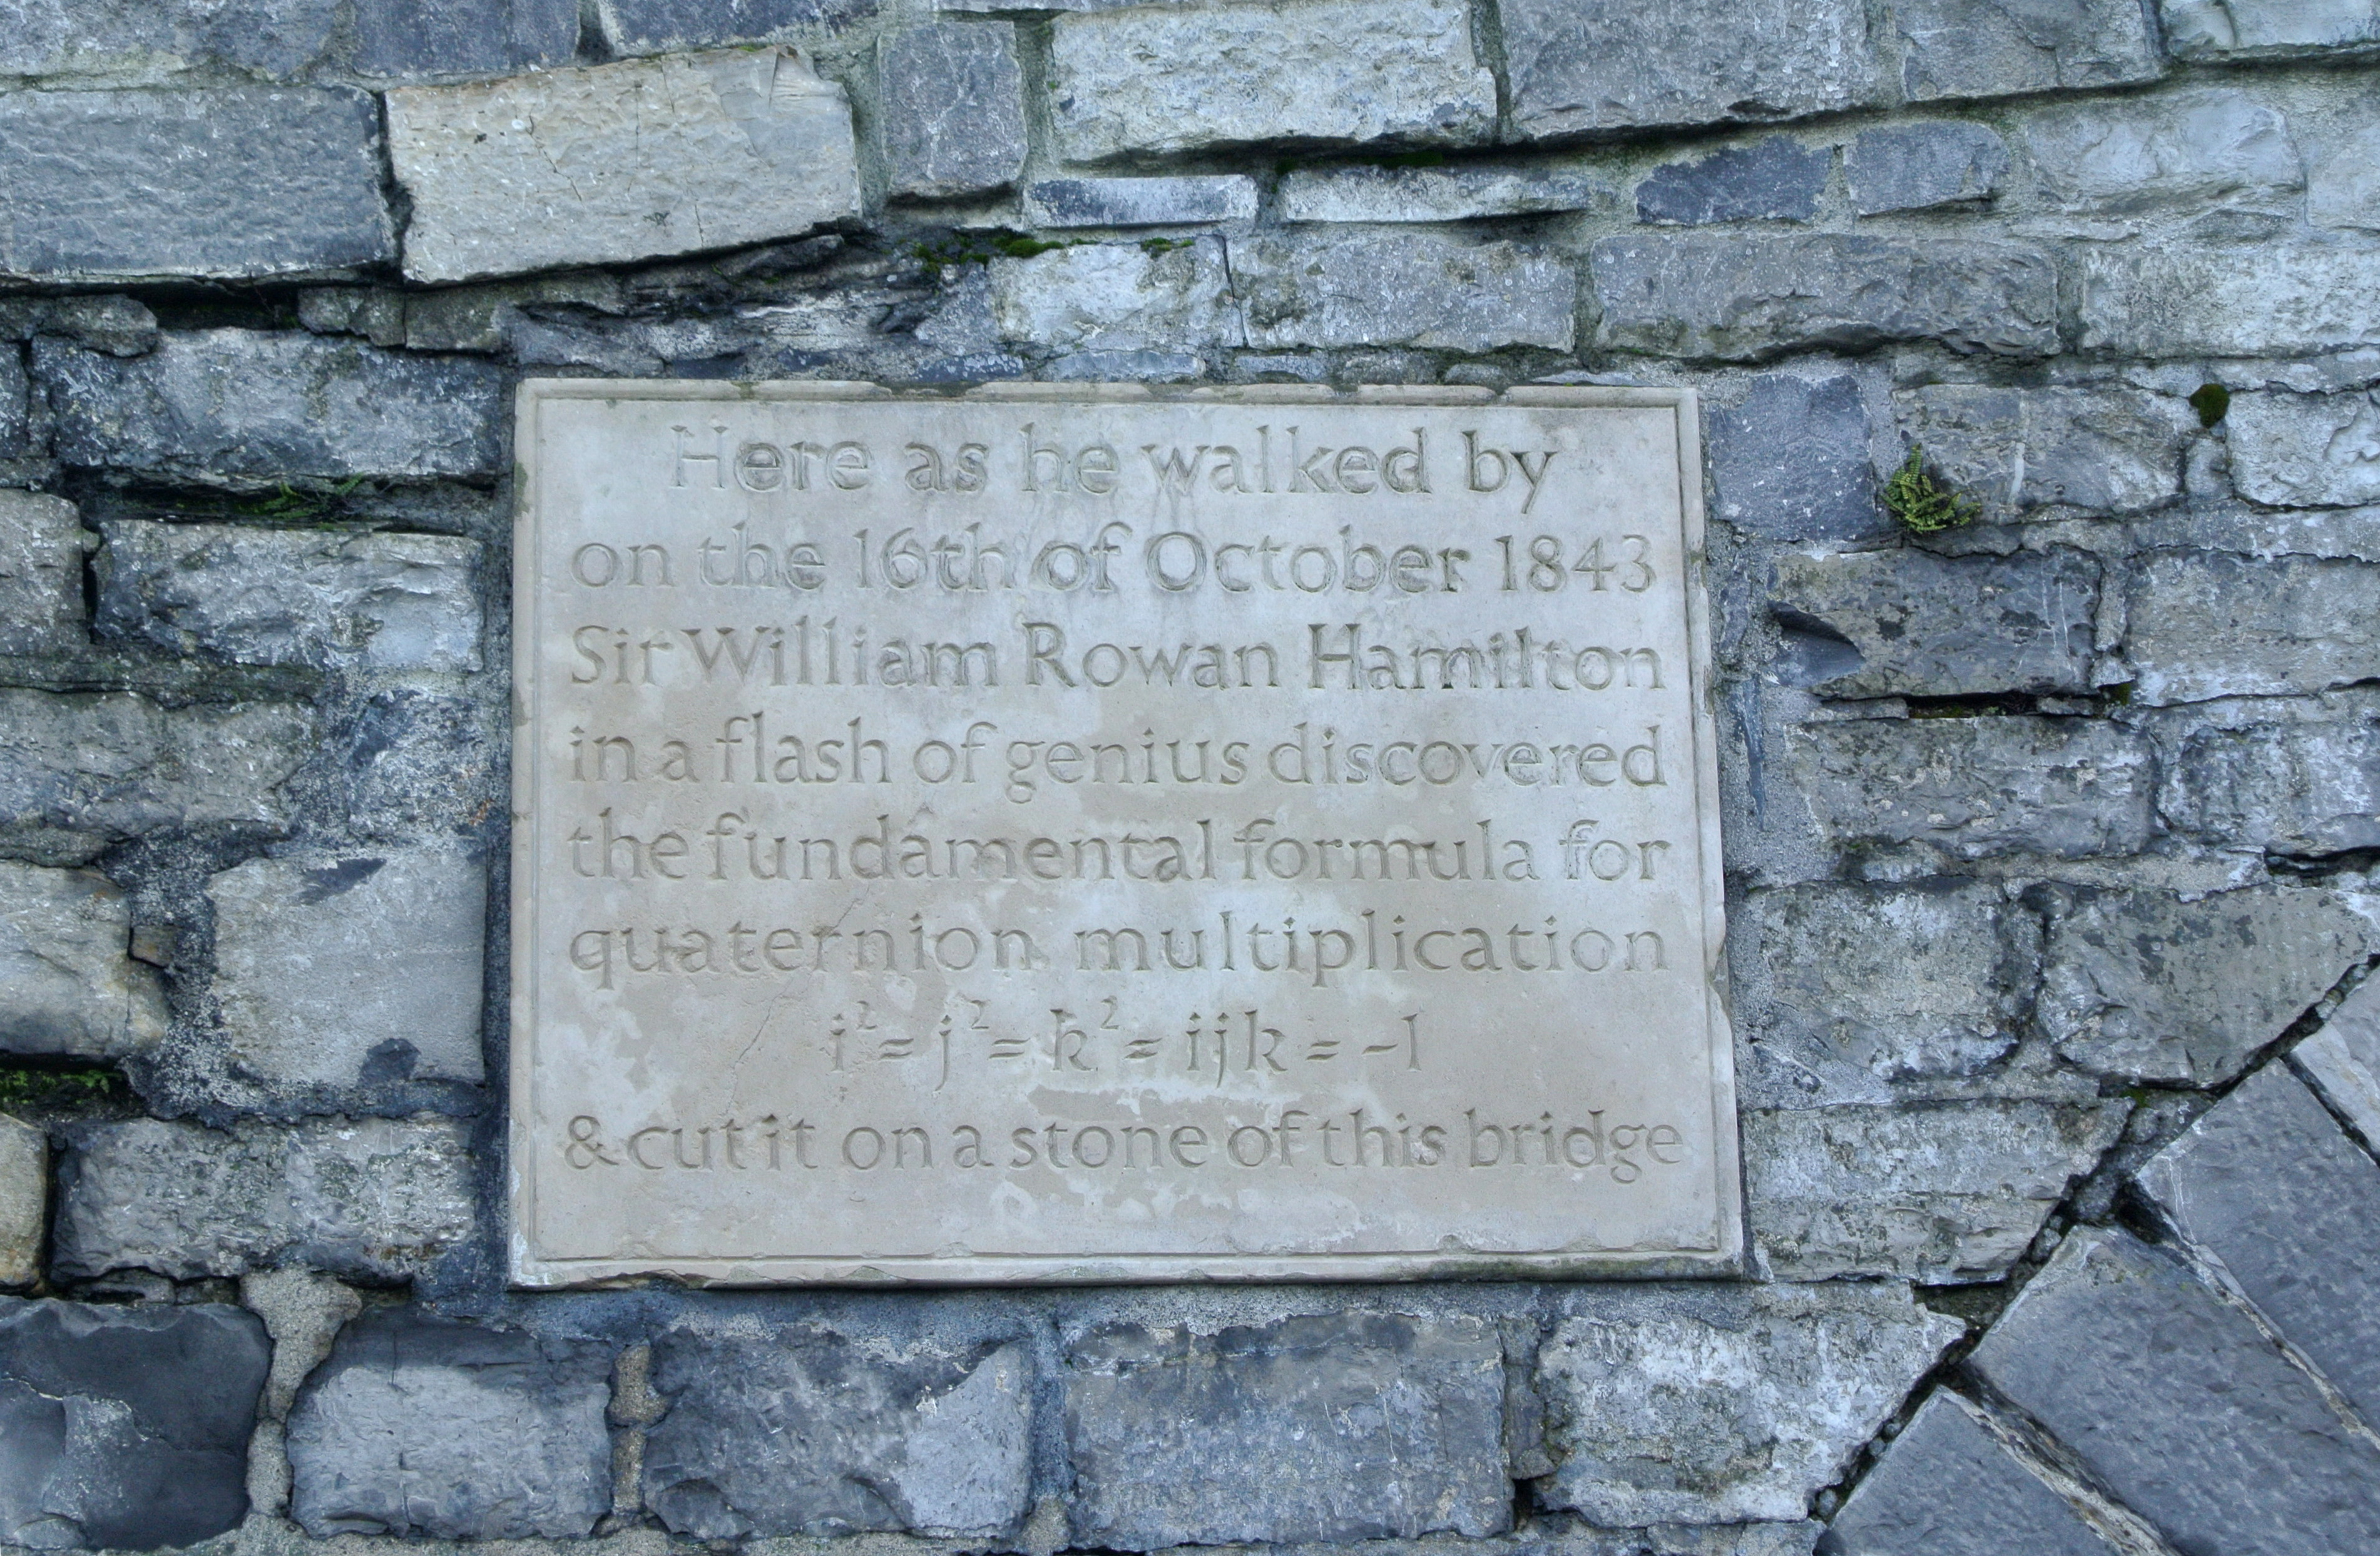
\includegraphics[width=0.90\textwidth]{./Figs/Fig_3.jpg}
\caption{Quaternion plaque on Brougham Bridge, Dublin \\ \ccbysa \href{https://commons.wikimedia.org/wiki/File:Inscription\_on\_Broom\_Bridge\_(Dublin)\_regarding\_the\_discovery\_of\_Quaternions\_multiplication\_by\_Sir\_William\_Rowan\_Hamilton.jpg}{Wikipedia - Cone83}}
\end{figure}
\end{column}

\begin{column}{0.50\columnwidth}
\begin{figure}[htbp]

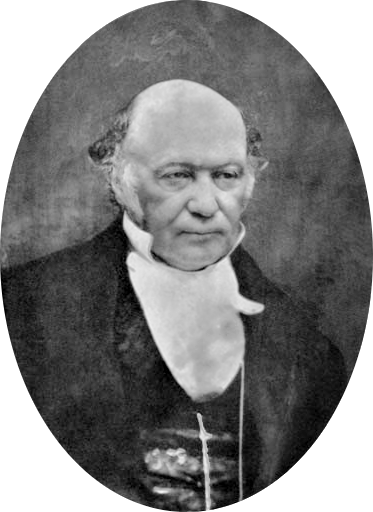
\includegraphics[height=0.60\textheight]{./Figs/Fig_4.png}
\caption{Portrait of Sir William Rowan Hamilton \\ \ccPublicDomainAlt \href{https://commons.wikimedia.org/wiki/File:William\_Rowan\_Hamilton\_portrait\_oval\_combined.png}{Wikipedia - Quibik}}
\end{figure}
\end{column}
\end{columns}
\end{frame}

\begin{frame}[label={sec:org1bcbdb8}]{Quaternions}
\begin{definition}[Quaternion]\label{sec:orga43bc3f}
\(\symbf{i}^2 = \symbf{j}^2 = \symbf{k}^2 = \symbf{ijk} = -1\)

\(\left\{ d + a\symbf{i} + b\symbf{j} + c\symbf{k} : a,b,c,d \in \symbb{R} \right\} \in \symbb{H}\)
\end{definition}

\begin{columns}
\begin{column}{0.50\columnwidth}
\begin{itemize}
\item<2-> \(\symbf{i}^2 = \symbf{ijk}\)

\begin{talign*}
  \symbf{i}^{-1} \symbf{i}^2 & = \symbf{i}^{-1} \symbf{ijk} \\
  \symbf{i} & = \symbf{jk}
\end{talign*}

\item<3-> \(\symbf{k}^2 = \symbf{ijk}\)

\begin{talign*}
  \symbf{k}^2 \symbf{k}^{-1} & = \symbf{ijk} \symbf{k}^{-1} \\
  \symbf{k} & = \symbf{ij}
\end{talign*}

\item<3-> \(\symbf{j} = \symbf{ki}\)
\end{itemize}
\end{column}

\begin{column}{0.50\columnwidth}
\begin{itemize}
\item<4-> \(\symbf{i} = \symbf{jk}\)

\begin{talign*}
  \symbf{ji} & = \symbf{jjk} \\
  \symbf{ji} & = \symbf{j}^2 \symbf{k} \\
  \symbf{ji} & = -\symbf{k} \\
  -\symbf{k} & = \symbf{ji}
\end{talign*}

\item<5-> \(-\symbf{i} = \symbf{kj}\)
\item<5-> \(-\symbf{j} = \symbf{ik}\)
\end{itemize}
\end{column}
\end{columns}
\end{frame}

\begin{frame}[label={sec:org83d92df}]{}
\begin{block}{Let,}
\(\symbf{i}^2 = \symbf{j}^2 = \symbf{k}^2 = \symbf{ijk} = -1\)

\(p = d + a\symbf{i} + b\symbf{j} + c\symbf{k}\)

\(q = w + x\symbf{i} + y\symbf{j} + z\symbf{k}\)
\end{block}

\begin{align*}
    p \ast q \only<1-2>{& = dw + dx\symbf{i} + dy\symbf{j} + dz\symbf{k} \\}
    \only<1-2>{& + aw\symbf{i} + ax\symbf{i}^2 + ay\symbf{ij} + az\symbf{ik} \\}
    \only<1-2>{& + bw\symbf{j} + bx\symbf{ji} + by\symbf{j}^2 + bz\symbf{jk} \\}
    \only<1-2>{& + cw\symbf{k} + cx\symbf{ki} + cy\symbf{kj} + cz\symbf{k}^2 \\}
    \only<2-3>{& = dw - ax - by - cz \\}
    \only<4>{& = dw - (ax + by + cz) \\}
    \only<5->{& = dw - \begin{asvector} a\\b\\c \end{asvector} \cdot \begin{asvector} x\\y\\z \end{asvector} \\}
    \only<2-5>{& + dx\symbf{i} + aw\symbf{i} + bz\symbf{i} - cy\symbf{i} \\}
    \only<2-5>{& + dy\symbf{j} - az\symbf{j} + bw\symbf{j} + cx\symbf{j} \\}
    \only<2-5>{& + dz\symbf{k} + ay\symbf{k} - bx\symbf{k} + cw\symbf{k} \\}
    \onslide<6->{& + \begin{avector}}
    \onslide<6->{dx + aw + bz - cy \\}
    \onslide<6->{dy - az + bw + cx \\}
    \onslide<6->{dz + ay - bx + cw}
    \onslide<6->{\end{avector}}
    \onslide<6->{\cdot \begin{avector} \symbf{i} \\ \symbf{j} \\ \symbf{k} \end{avector} \\}
    \onslide<7->{& = dw - \begin{asvector} a\\b\\c \end{asvector} \cdot \begin{asvector} x\\y\\z \end{asvector} + \left(d \begin{asvector} x\\y\\z \end{asvector} \only<8->{+ w \begin{asvector} a\\b\\c \end{asvector}} \only<9->{+ \begin{asvector} a\\b\\c \end{asvector} \times \begin{asvector} x\\y\\z \end{asvector}} \only<7-8>{\cdots} \right) \cdot \begin{asvector} \symbf{i}\\\symbf{j}\\\symbf{k} \end{asvector}}
\end{align*}
\end{frame}

\section{Quaternion Iterative Methods}
\label{sec:org68f0ace}

\begin{frame}[label={sec:org5fabcdb},fragile]{Implementation}
 \begin{block}{Quaternion Multiplication}
\begin{lstlisting}[language=Python,firstnumber=1,numbers=left]
def q_mult(p, q):
    r = Quat(
        p.w*q.w – p.x*q.x – p.y*q.y - p.z*q.z,
        p.w*q.x + p.x*q.w + p.y*q.z - p.z*q.y,
        p.w*q.y – p.x*q.z + p.y*q.w + p.y*q.x,
        p.w*q.z + p.x*q.y – p.y*q.x + p.z*q.w
    )
    return r
\end{lstlisting}
\end{block}
\end{frame}

\begin{frame}[label={sec:orgad19de7},fragile]{Implementation}
 \begin{block}{Quaternion Square}
\begin{lstlisting}[language=Python,firstnumber=1,numbers=left]
def q_square(q):
    r = Quat(
        q.w*q.w – q.x*q.x – q.y*q.y - q.z*q.z,
        2*q.w*q.x,
        2*q.w*q.y,
        2*q.w*q.z
    )
    return r
\end{lstlisting}
\end{block}
\end{frame}

\begin{frame}[label={sec:orgbe93d52},fragile]{Implementation}
 \begin{columns}
\begin{column}{0.45\columnwidth}
\begin{block}{Quaternion Add}
\begin{lstlisting}[language=Python,firstnumber=1,numbers=left]
def q_add(p, q):
    r = Quat(
        p.w + q.w,
        p.x + q.x,
        p.y + q.y,
        p.z + q.z
    )
    return r
\end{lstlisting}
\end{block}
\end{column}

\begin{column}{0.45\columnwidth}
\begin{block}<2->{Quaternion Magnitude}
\begin{lstlisting}[language=Python,firstnumber=1,numbers=left]
def q_abs(q):
    return q.w*q.w +
           q.x*q.x +
           q.y*q.y +
           q.z*q.z
\end{lstlisting}
\end{block}
\end{column}
\end{columns}
\end{frame}

\begin{frame}[label={sec:orgca04647},fragile]{Implementation}
 \begin{block}{Iteration}
\begin{lstlisting}[language=Python,firstnumber=1,numbers=left]
N = 12
B = 16
q = Quat(-0.2, 0.4, -0.4, -0.4)
def iterate(z):
    for n in range(N):
        z = q_add(q_square(z), q)
        if q_abs(z) > B*B: break
    return n
\end{lstlisting}
\end{block}
\end{frame}

\begin{frame}[label={sec:org9fd9caa}]{Iteration}
\begin{columns}
\begin{column}{0.5\columnwidth}
\begin{block}{Rules}
\(f(z) = z^2 + 0.3 - 0.375\symbf{i} - 0.675\symbf{j} - 0.112\symbf{k}\)

\(z_0 = 0.5 - 0.5\symbf{i} + 0.5\symbf{j} - 0.5\symbf{k}\)
\end{block}

\begin{itemize}[<+->]
\item \(f^0(z) = 0.5 - 0.5\symbf{i} + 0.5\symbf{j} - 0.5\symbf{k}\)
\item \(f^1(z) = -0.2 - 0.875\symbf{i} - 0.175\symbf{j} - 0.612\symbf{k}\)
\item \(f^2(z) = -0.831 - 0.025\symbf{i} - 0.605\symbf{j} + 0.133\symbf{k}\)
\item \(f^3(z) \approx 0.6066 - 0.333\symbf{i} + 0.330\symbf{j} - 0.333\symbf{k}\)
\item \(f^4(z) \approx 0.336 - 0.779\symbf{i} - 0.274\symbf{j} - 0.515\symbf{k}\)
\item \(f^5(z) \approx -0.535 - 0.899\symbf{i} - 0.860\symbf{j} - 0.458\symbf{k}\)
\end{itemize}
\end{column}

\begin{column}{0.5\columnwidth}
\begin{center}
\includegraphics<1>[width=.9\linewidth]{Figs/exports/Iter_5-0.png}
\includegraphics<2>[width=.9\linewidth]{Figs/exports/Iter_5-1.png}
\includegraphics<3>[width=.9\linewidth]{Figs/exports/Iter_5-2.png}
\includegraphics<4>[width=.9\linewidth]{Figs/exports/Iter_5-3.png}
\includegraphics<5>[width=.9\linewidth]{Figs/exports/Iter_5-4.png}
\includegraphics<6>[width=.9\linewidth]{Figs/exports/Iter_5-5.png}
\end{center}
\end{column}
\end{columns}
\end{frame}

\begin{frame}[label={sec:org6b8319a},b]{Plotting}
\begin{columns}
\begin{column}{0.5\columnwidth}
\begin{figure}[htbp]
\centering
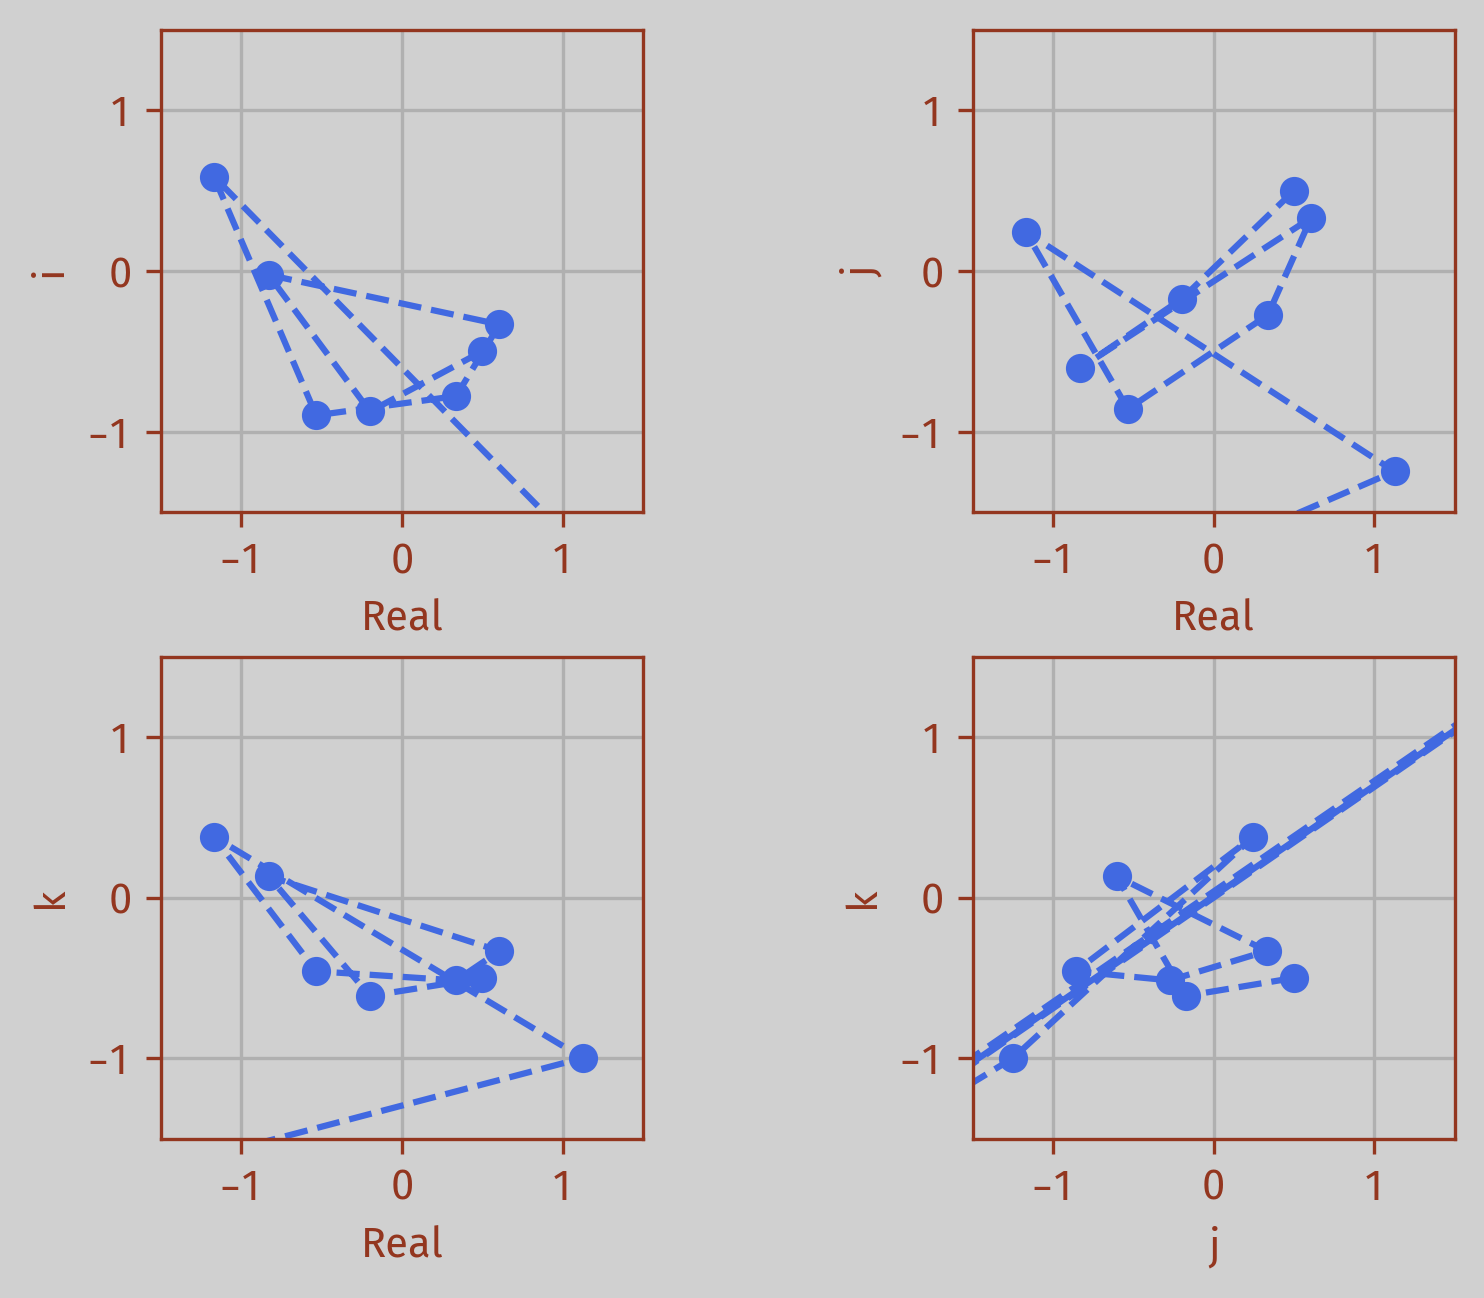
\includegraphics[width=0.75\textwidth]{Figs/exports/Iter_5-12.png}
\caption{\(f(z) = z^2 + 0.3 - 0.375\symbf{i} - 0.675\symbf{j} - 0.112\symbf{k}\) \\ \(f^{12}(0.5 - 0.5\symbf{i} + 0.5\symbf{j} - 0.5\symbf{k})\)}
\end{figure}
\end{column}

\begin{column}{0.5\columnwidth}
\begin{figure}[htbp]
\centering
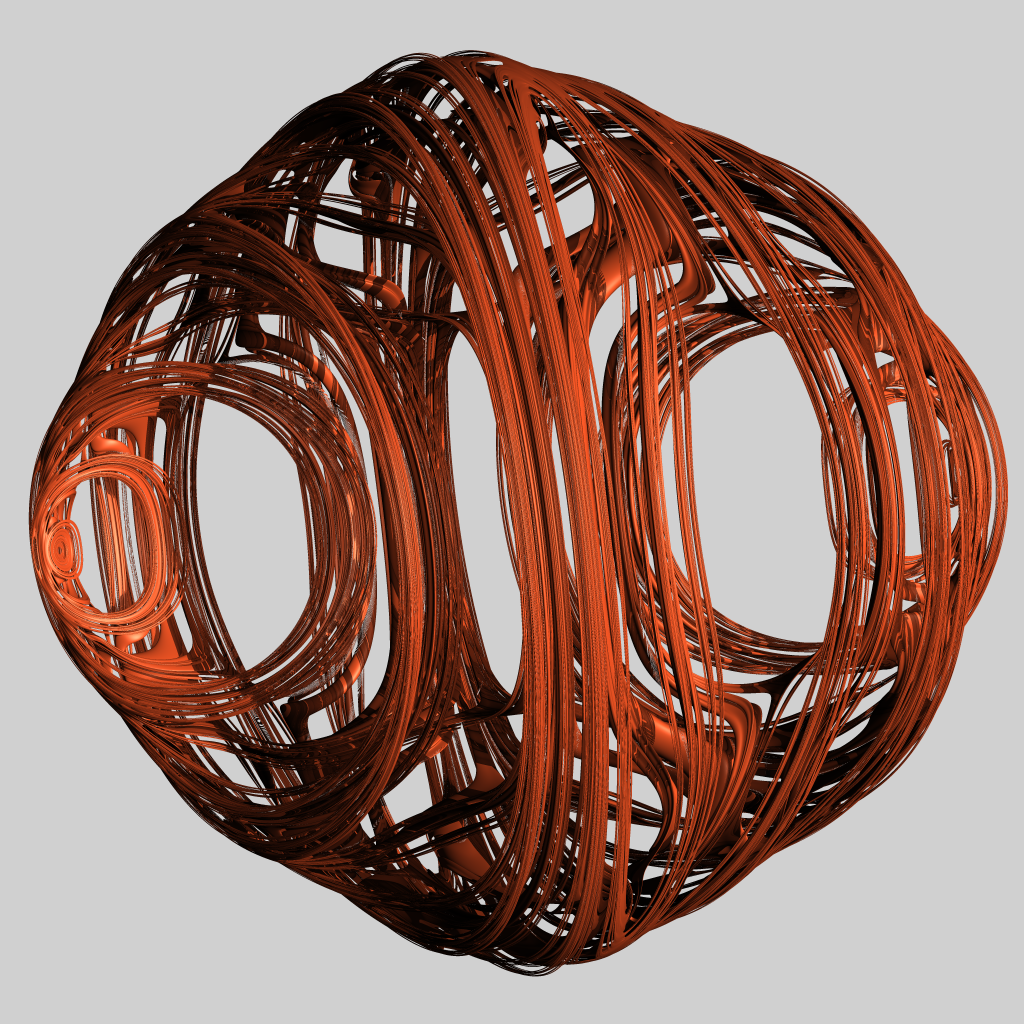
\includegraphics[width=0.75\textwidth]{./Figs/Fig_1v2.png}
\caption{\(f(z) = z^2 + 0.3 - 0.375\symbf{i} - 0.675\symbf{j} - 0.112\symbf{k}\) \\ Axis: Real, \(\symbf{i}, \symbf{j}\)}
\end{figure}
\end{column}
\end{columns}
\end{frame}

\begin{frame}[label={sec:org4327878}]{Ray Tracing}
\begin{figure}[htbp]

\includesvg[height=0.60\textheight]{./Figs/Fig_5-1}
\caption{Ray Tracing Diagram \\ \ccbysa \href{https://commons.wikimedia.org/wiki/File:Ray\_trace\_diagram.svg}{Wikipedia - Henrik} with modifications}
\end{figure}
\end{frame}

\begin{frame}[label={sec:org4c509f6}]{Ray Marching}
\begin{columns}
\begin{column}{0.5\columnwidth}
\begin{figure}[htbp]

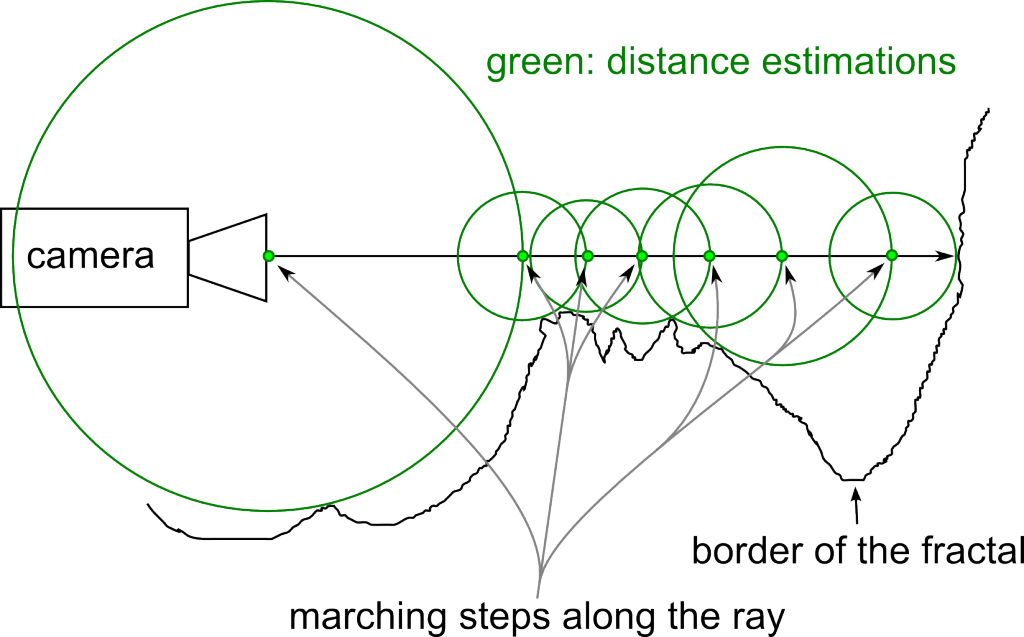
\includegraphics[width=.9\linewidth]{./Figs/Fig_6.png}
\caption{Ray Marching \\ \ccCopy \href{http://celarek.at/2014/05/real-time-3d-mandelbulb/}{Adam Celarek}}
\end{figure}
\end{column}

\begin{column}{0.5\columnwidth}
\begin{theorem}[Distance Estimation]\label{sec:org247c76f}
Let \(f(z) = z^m + q\) where \(q \in \symbb{H}, m \in \symbb{Z}^+\) be the iterative function of a Julia fractal. Then, the distance, \(\delta\), to the fractal can be approximated by
\begin{align*}
    a \frac{z_n}{z_n'} < \delta
\end{align*}
where \(a \in \symbb{R}\) is some constant coefficient.
\end{theorem}
\end{column}
\end{columns}
\end{frame}

\begin{frame}[label={sec:org63dfbe9}]{Normal Estimation}
\begin{figure}[htbp]

\includesvg[height=0.60\textheight]{./Figs/Fig_5-2}
\caption{Ray Tracing Diagram \\ \ccbysa \href{https://commons.wikimedia.org/wiki/File:Ray\_trace\_diagram.svg}{Wikipedia - Henrik} with modifications}
\end{figure}
\end{frame}

\begin{frame}[label={sec:org963bc90}]{Quaternion Iterative Fractals}
\begin{columns}
\begin{column}{0.55\columnwidth}
\begin{block}{Quaternion Juila Set Example}
\begin{itemize}
\item Defined by iterative function in 4D Quaternion space
\end{itemize}
\end{block}
\end{column}

\begin{column}{0.45\columnwidth}
\begin{figure}
\animategraphics[autoplay,interpolate,width=0.75\textwidth,loop,palindrome]{2}{Figs/Iter_Q/}{1}{11}
\caption{\(f(z) = z^2 + 0.3 - 0.375\symbf{i} - 0.675\symbf{j} - 0.112\symbf{k}\) \\ Axis: Real, \(\symbf{i}, \symbf{j}\) \\ N = 1-11}
\end{figure}
\end{column}
\end{columns}
\end{frame}

\begin{frame}[label={sec:org781f8bb}]{Summary}
\setcounter{tocdepth}{2}
\tableofcontents
\end{frame}

\begin{frame}[allowframebreaks,label=]{References}
\nocite{*}
\bibliography{sources}
\bibliographystyle{alpha}
\end{frame}

\begin{frame}[label={sec:orgb021ad5}]{Questions?}
\begin{center}
\url{https://github.com/scrufulufugus/senior-synthesis}


\includegraphics[height=0.70\textheight]{./Figs/qr.png}
\end{center}
\end{frame}
\end{document}